\documentclass[letterpaper, 11pt]{article}
\usepackage{fullpage}
\usepackage{authblk}
\usepackage{amsmath}
\usepackage{amssymb}
\usepackage{bm}
\usepackage{lineno}
\usepackage{graphicx}

%%%%%%%%%%%%%%%%%%%%%%%%%%%%%%%%%%%%%%%%%%%%%%%%%%%%%%%%%%%%%%
\begin{document}

\title{ECE750 Report}
\author{Arthur}
\author{Daniel}
\affil{University of Waterloo}
\date{Dec 4, 2024}
\maketitle

%%%%%%%%%%%%%%%%%%%%%%%%%%%%%%%%%%%%%%%%%%%%%%%%%%%%%%%%%%%%%%
\begin{abstract}
    
    Lecture abstract section.
\end{abstract}
%%%%%%%%%%%%%%%%%%%%%%%%%%%%%%%%%%%%%%%%%%%%%%%%%%%%%%%%%%%%%%
\section{Introduction}\label{s:intro}
%%%%%%%%%%%%%%%%%%%%%%%%%%%%%%%%%%%%%%%%%%%%%%%%%%%%%%%%%%%%%%
\section{doc}
Here is an inline equation $a=b$. Below is not inline equation, but only one line.
\[
a = b = c.\\
f(x) = x_{\Delta}^2  + \gamma.
f(x) = \frac{numerators}{denominators}
\]

Below is multiple-line equations as \ref{e:fx}.
\begin{equation}\label{e:fx}
    f(x) = \left(\sum_a^ba+b\right)   \\ 
    x = \sin(x)
\end{equation}

Below is an example of alignment.
\begin{align}
    f(x) &= x + 5 \\
    y &= y - 8
\end{align}

Below is a table.
\begin{table}[h]
    \caption{HiPs tree lengthscales and timescales.}
    \label{t:hips_scales}
    \centering
    \begin{tabular}{l l l}
        \hline
        Level & Length scale  &Time scales \\
        \hline
        0  & $L_0$      & $\tau _0$     \\
        1 & $L_9/{2}$    & $\tau_0/2^{2/3}$    \\
        2   & $L_0/4$    & $\tau_0/4^{2/3}$ \\
        $\ldots$  & $\ldots$ & $\ldots$  \\ 
        \hline 
        
    \end{tabular}
\end{table}

Below is a fiture.
\begin{figure}[htpb]
    \centering
    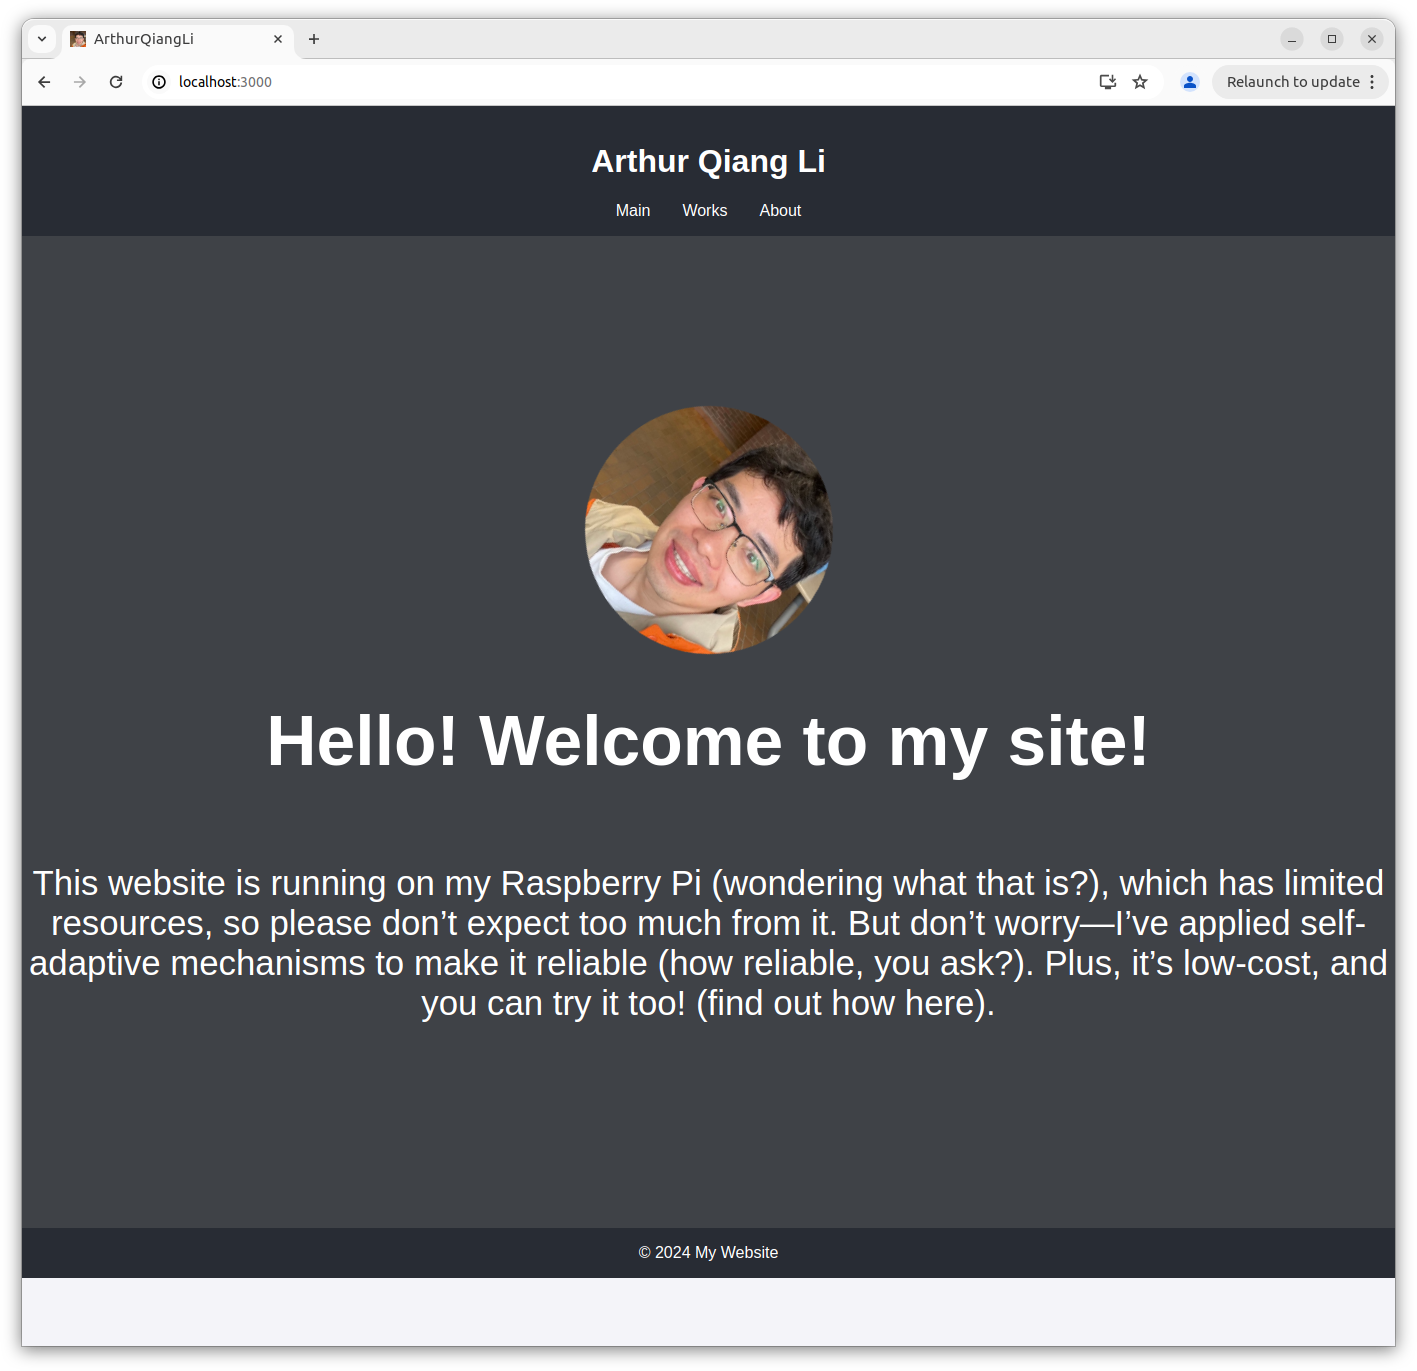
\includegraphics[width=3in]{./media/Screenshot from 2024-11-11 00-41-15.png}
    \caption{the name of this fiture.}
    \label{f:homepage}
\end{figure}

%%%%%%%%%%%%%%%%%%%%%%%%%%%%%%%%%%%%%%%%%%%%%%%%%%%%%%%%%%%%%%
\section{Methods}

\subsection{Numerics}
 
what ever content. As shown in Section \ref{s:intro}, this is the cite at \cite{LIGNELL_2007A, Bockhorn_1994} end.


%%%%%%%%%%%%%%%%%%%%%%%%%%%%%%%%%%%%%%%%%%%%%%%%%%%%%%%%%%%%%%

\bibliographystyle{unsrt}
\bibliography{r1}
\end{document}


